\documentclass[11pt]{article}
\usepackage[spanish]{babel}

\usepackage{amssymb}
\usepackage{enumerate}
\usepackage{geometry}
\usepackage{mathtools}
\usepackage{multicol}
\usepackage{soul}

\usepackage{graphicx}
	\graphicspath{ {assets/} }


%%%%%%%%%%%%%%%%%%%%%%%%%%%%%%%%%%
%%%%%%%%%%%%%%%%%%%%%%%%%%%%%   %%
%%        Datos Trabajo     %%  %%
%%%%%%%%%%%%%%%%%%%%%%%%%%%%%%%%%%

\newcommand{\titulo}[0]{
Actividad 3. Método de Gauss}
\newcommand{\materia}[0]{\'Algebra Lineal}
\newcommand{\grupo}[0]{BI-BALI-2002-B1-012}
\newcommand{\unidad}[0]{Unidad 2}


%%%%%%%%%%%%%%%%%%%%%%%%%%%%%%%%%%
%%%%%%%%%%%%%%%%%%%%%%%%%%%%%%%%%%

\usepackage[pdftex,
            pdfauthor={bench},
            pdftitle={\titulo},
            pdfsubject={\materia},
            pdfkeywords={\grupo, \unidad, UnADM},
            pdfproducer={Latex with hyperref, or other system},
            pdfcreator={pdflatex, or other tool}]{hyperref}
%%%%%%%%%%%%%%%%%%%%%%%%%%%%%%%%%%
%%%%%%%%%%%%%%%%%%%%%%%%%%%%%%%%%%

\title{
	
\includegraphics{../../../assets/logo-unadm} \\
	\ \\ Benjam\'in Rivera \\
	\bf{\titulo}\\\ \\}

\author{
	Universidad Abierta y a Distancia de México \\
	TSU en Biotecnolog\'ia \\
	\textit{Materia:} \materia \\
	\textit{Grupo:} \grupo \\
	\textit{Unidad:} \unidad \\
	\\
	\textit{Matricula:} ES202105994 }

\date{\textit{Fecha de entrega:} \today}


%%%%%%%%%%%%%%%%%%%%%%%%%%%%%
%%        Documento         %%
%%%%%%%%%%%%%%%%%%%%%%%%%%%%%%%
\begin{document}
\maketitle\newpage

%%%%%%%%%%%%%%%%%%%%%%%%%%%%%%%%
%%          Actividad          %%
%%%%%%%%%%%%%%%%%%%%%%%%%%%%%%%%%%
	\par Resuelve los siguientes sistemas de ecuaciones utilizando el \textit{m\'etodo de \textbf{Gauss}}, para hacer seguiremos la siguiente lista de pasos:
	\begin{enumerate}
		\item Normalizaremos el sistema
		\item Representaremos el sistema como matriz ampliada
		\item Se conviera la matriz ampliada en matriz triangular superior
		\item Calculamos $x_1, x_2 \text{ y } x_3$
	\end{enumerate}
	durante el ejercicio usaremos $M_n$ para referirnos a la fila $n$ de la matriz $M$.

\begin{multicols}{2}
	\begin{enumerate}[\bf{Sistema} 1]
		\item 
			\ \\$\begin{matrix}
				2x + 7y + 6z = 48 \\
				4x + 5y + 9z = 24 \\
				3x +  y – 2z = 14 \\
			\end{matrix}$
		
			Dado que la matriz ya esta normalizada, podemos pasar a mostrar la matriz ampliada
				$$M = \left(\begin{array}{rrrr}
						2 & 7 & 6 & 48 \\
						4 & 5 & 9 & 24 \\
						3 & 1 & -2 & 14
					\end{array}\right)$$
			Ahora, para obtener la matriz triangular superior primero haremos $M_2 = M_2 - 2*M_1$ y $M_3 = M_3 - \frac{3}{2}M_1$, de donde queda 
				$$\left(\begin{array}{rrrr}
						2 & 7 & 6 & 48 \\
						0 & -9 & -3 & -72 \\
						0 & -\frac{19}{2} & -11 & -58
					\end{array}\right)$$
			luego hacemos que $M_3 = M_3 - \frac{19}{18} M_2$
				$$\left(\begin{array}{rrrr}
						2 & 7 & 6 & 48 \\
						0 & -9 & -3 & -72 \\
						0 & 0 & -\frac{47}{6} & 18
					\end{array}\right)$$
			multiplicamos $M_2 = M_2* \frac{-1}{3}$ y a $M_3 = M_3*-6$ de manera que
				$$\left(\begin{array}{rrrr}
					2 & 7 & 6 & 48 \\
					0 & 3 & 1 & 24 \\
					0 & 0 & 1 & \frac{-108}{47}
				\end{array}\right)$$
			ahora sabemos que $$z = -\frac{108}{47} \sim -2.29787234043$$ y con z  podmos obtener que
				\begin{eqnarray*}
					3y + z &=& 24 \\
					3y &=& 24 - z \\
					y &=& 8- \frac{z}{3} \\
					y &=& 8 - \frac{-108/47}{3} \\
					y &=& \frac{412}{47} \sim 8.76595744681
				\end{eqnarray*}
			y que como ya conocemos $z,y$, entonces para $x$ tenemos que
				\begin{eqnarray*}
					2x + 7y + 6z &=& 48 \\
					2x &=& 48 - 7y - 6z \\
					x  &=& 24 - \frac{7}{2}y - 3z \\
					x  &=& \frac{10}{47} \sim 0.21276595744
				\end{eqnarray*}

		\item
			\ \\ $\begin{matrix}
				x + 12y + 3z = 19 \\
				4 +  5y + 6z = 24 \\
				3 +  7y + 2z = 4
			\end{matrix}$
			
			\par Primero pasamos la matriz a su forma normal, de esto queda
			$$\begin{matrix}
				1x + 12y + 3z = 19 \\
				0x +  5y + 6z = 20 \\
				0x +  7y + 2z = 1
			\end{matrix}$$
			
			ahora si con eso generamos la matriz extendida
			
			$$\left(\begin{array}{rrrr}
				1 & 12 & 3 & 19 \\
				0 & 5 & 6 & 20 \\
				0 & 7 & 2 & 1
			\end{array}\right)$$
			
 			ahora, para pasar a matriz trangular hacemos que la $M_3$ sea -7/5 veces la $M_2$ mas la $M_3$
			
			$$\left(\begin{array}{rrrr}
				1 & 12 & 3 & 19 \\
				0 & 5 & 6 & 20 \\
				0 & 0 & -\frac{32}{5} & -27
			\end{array}\right)$$
			
			y ahora arreglamos $M_3 = M_3 * -5/32$ para que nos quede
			
			$$\left(\begin{array}{rrrr}
				1 & 12 & 3 & 19 \\
				0 & 5 & 6 & 20 \\
				0 & 0 & 1 & \frac{135}{32}
			\end{array}\right)$$
			
			de lo anterior vemos que $$z = \frac{135}{32} \sim 4.21875$$ y con eso podemos
			
			\begin{eqnarray*}
				5y + 6z &=& 20 \\
				5y &=& 20 - 6z \\
				y &=& 4 - \frac{3}{2}z = \frac{-17}{16} \sim -1.0625
			\end{eqnarray*}
			
			y de una manera similar obtenemos que 
			
			\begin{eqnarray*}
				x + 12y + 3z &=& 19 \\
				x &=& 19 - 12y - 3z \\
				x &=& \frac{611}{32} \sim -19.09375
			\end{eqnarray*}
			
			
			
		\item
			\ \\ $\begin{matrix}
				x - 2y + 4z =  7 \\
				4 + 2y - 8z = 10 \\
				2 + 5y + 7z = 23
			\end{matrix}$
			
			\par Primero normalizamos el sistema, de manera que quede		
			$$\begin{matrix}
				1x - 2y + 4z =  7 \\
				0x + 2y - 8z =  6 \\
				0x + 5y + 7z = 21
			\end{matrix}$$
			
			luego procedemos a expresar la matriz expandida
			
			$$\left(\begin{array}{rrrr}
				1 & -2 & 4 & 7 \\
				0 & 2 & -8 & 6 \\
				0 & 5 & 7 & 21
			\end{array}\right)$$
			
			y para hacerla triangular hacemos que la $M_3$ sea -5/2 veces la $M_2$ mas la $M_3$
			
			$$\left(\begin{array}{rrrr}
				1 & -2 & 4 & 7 \\
				0 & 2 & -8 & 6 \\
				0 & 0 & 27 & 6
			\end{array}\right)$$
			
			arreglamos un poco $M_2 = M_2/2$ y $M_3 = M_3/27$ de manera que
			
			$$\left(\begin{array}{rrrr}
				1 & -2 & 4 & 7 \\
				0 & 1 & 4 & 3 \\
				0 & 0 & 1 & \frac{6}{27}
			\end{array}\right)$$
			
			 y al final, con un procedimiento similar al anterior, vemos que las soluciones son
			 \begin{eqnarray*}
			 	x &=& \frac{125}{9} \sim 13.8888888889\\
			 	y &=& \frac{35}{9} \sim 3.88888888889\\
			 	z &=& \frac{2}{9} \sim 0.22222222222
			 \end{eqnarray*}
			
	\end{enumerate}
\end{multicols}




	\subsection*{Comprobaci\'on}
	\par Para corroborar los resutlados se uso el \textit{CAS} 
\footnote{Sistema Algebraico Computacional, por sus siglas en ingles} 
	\href{https://www.sagemath.org/}{SageMath}, que utiliza como interfaz el lenguaje de programaci\'on \href{https://www.python.org/}{Python} y la \textit{UI} jupyter. El archivo html resultante del notebook generado se puede consultar \href{https://github.com/BenchHPZ/UnADM-Biotecnologia/blob/master/B1-1/AL/Actividades/BALI_U2_A3_BERC.ipynb}{aqu\'i}.
	
	\begin{figure}[h]
		\centering
		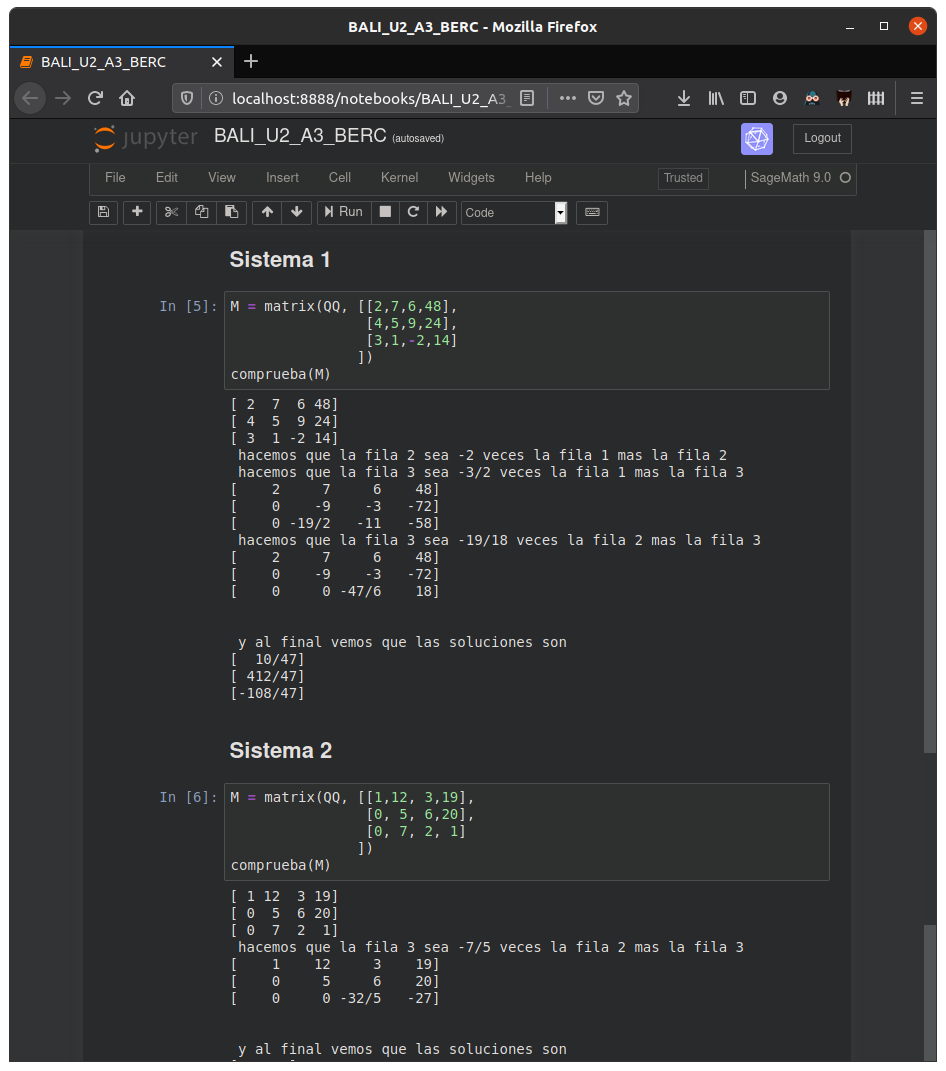
\includegraphics[width=0.49\textwidth]{BALI-U2-A3-1.png}
		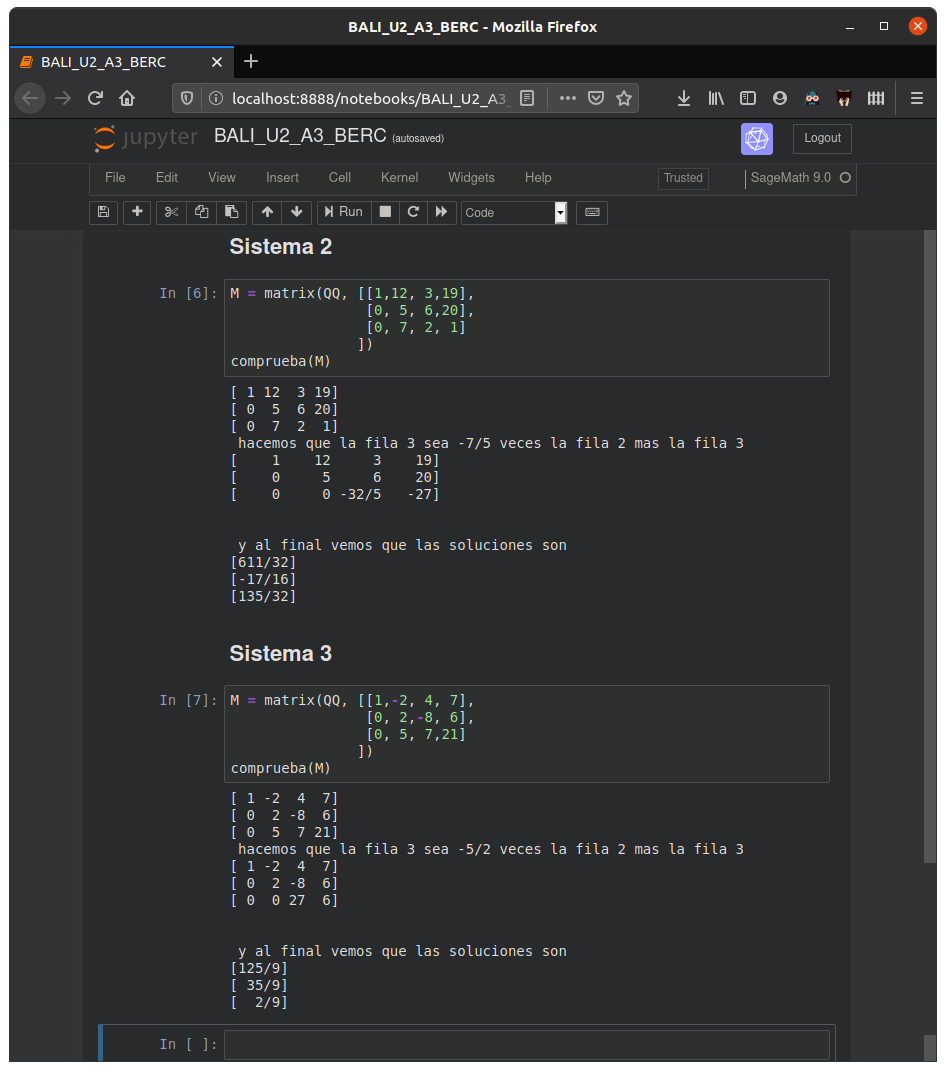
\includegraphics[width=0.49\textwidth]{BALI-U2-A3-2.png}
		\caption{Comprobaci\'on de ejercicio 1, 2 y 3}
	\end{figure}


%%%%%%%%%%%%%%%%%%%%%%%%%%%%%%%%
%%         Bibliografia        %%
%%%%%%%%%%%%%%%%%%%%%%%%%%%%%%%%%%

\newpage
\begin{thebibliography}{X}
	\bibitem{biblio} UnADM. (S/D). \emph{Primer semestre Algebra Lineal}. \today, de Universidad Abierta y a Distancia de México \textbar{} DCSBA Sitio web: \url{https://dmd.unadmexico.mx/contenidos/DCSBA/BLOQUE1/BI/01/BALI/unidad_01/descargables/BALI_U1_Contenido.pdf}
\end{thebibliography}

\end{document}